\documentclass[conference]{IEEEtran}
\usepackage{cite}
\usepackage{amsmath,amssymb,amsfonts}
\usepackage{graphicx}
\usepackage{hyperref}
\usepackage{textcomp}
\usepackage{xcolor}
\def\BibTeX{{\rm B\kern-.05em{\sc i\kern-.025em b}\kern-.08em
    T\kern-.1667em\lower.7ex\hbox{E}\kern-.125emX}}
\setcounter{MaxMatrixCols}{12} % increase maximum matrix width
\begin{document}

\title{Application of LDPC Codes In Computer Memory\\
{\large ELEC 433 Final Project}
}

\author{\IEEEauthorblockN{Tom Wang}
\and
\IEEEauthorblockN{Natalie Balashov}
}

\maketitle

\begin{abstract}
  TODO: add short abstract here.
\end{abstract}

\section{Introduction}
TODO: add introduction here

\section{LDPC Codes}
LDPC codes, or low-density parity-check codes, are a class of linear block codes that are characterized by sparse parity-check matrices.
The sparsity of the parity-check matrix allows for efficient encoding and decoding algorithms.
LDPC codes are also known to achieve near Shannon capacity performance when decoded using iterative message-passing algorithms.

\subsection{Types of LDPC Codes}
There are two main types of LDPC codes: regular and irregular.
Regular LDPC codes have a constant column weight and row weight, while irregular LDPC codes have varying column and row weights.
Regular LDPC codes are easier to analyze and implement, but irregular LDPC codes can achieve better performance.

Gallager developed the LDPC code as his Ph.D. thesis in 1962.
The parity-check matrix of a regular LDPC code is defined by the following equation:

A regular LDPC code $(j,i)$ has a weight of $j$ for each column and a weight of $i$ for each row.\ref{[1]}

An example of a parity-check matrix for a regular LDPC code where $j=3$ and $i=4$ is shown below:

$$\begin{bmatrix}
  1 & 1 & 1 & 1 & 0 & 0 & 0 & 0 & 0 & 0 & 0 & 0\\
  0 & 0 & 0 & 0 & 1 & 1 & 1 & 1 & 0 & 0 & 0 & 0\\
  0 & 0 & 0 & 0 & 0 & 0 & 0 & 0 & 1 & 1 & 1 & 1\\
  1 & 0 & 0 & 0 & 1 & 0 & 0 & 0 & 1 & 0 & 0 & 0\\
  0 & 1 & 0 & 0 & 0 & 1 & 0 & 0 & 0 & 1 & 0 & 0\\
  0 & 0 & 1 & 0 & 0 & 0 & 1 & 0 & 0 & 0 & 1 & 0\\
  0 & 0 & 0 & 1 & 0 & 0 & 0 & 1 & 0 & 0 & 0 & 1\\
  1 & 1 & 0 & 0 & 0 & 0 & 1 & 1 & 0 & 0 & 0 & 0\\
  0 & 0 & 1 & 1 & 0 & 0 & 0 & 0 & 1 & 1 & 0 & 0\\
  0 & 0 & 0 & 0 & 1 & 1 & 0 & 0 & 0 & 0 & 1 & 1
\end{bmatrix}$$

So this is a $(3,4)$ regular LDPC code where the column weight is 3 and the row weight is 4. The dimension of the code is $n=12$ and $n-k=9$.

The rate $R=1-\frac{j}{i}=\frac{k}{n}=\frac{1}{4}$.

Irregular LDPC codes have varying column and row weights.
However, they are distributed uniformly across the parity-check matrix.
Irregular LDPC codes can achieve better performance than regular LDPC codes, but they are more difficult to analyze and implement.

\subsection{Tanner Graphs}
A Tanner graph is a bipartite graph that represents the parity-check matrix of an LDPC code. The Tanner graph consists of two sets of nodes: variable nodes and check nodes. The edges of the graph connect variable nodes to check nodes and vice versa.

The Tanner graph is used to visualize the structure of the LDPC code and to develop efficient decoding algorithms.

For example, for this matrix: \[
    \begin{bmatrix}
        1 & 1 & 0 & 0\\
        1 & 0 & 1 & 1
    \end{bmatrix}
\]

The Tanner graph is shown below:

\begin{figure}[htbp]
\centerline{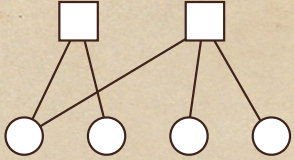
\includegraphics{Images/tanner_graph.png}}
\caption{Example of a figure caption.}
\label{fig}
\end{figure}

In Fig. \ref{fig}, we see that there are two parity nodes.

A \textbf{cycle} in a Tanner graph is a closed path that starts and ends at the same node.

A \textbf{girth} of a Tanner graph is the length of the shortest cycle in the graph. A larger girth is desirable because it leads to better error-correction performance.

\subsection{Encoding and Generator Matrices}
Given a parity-check matrix $H$ for an LDPC code, the generator matrix $G$ can be constructed using the following steps:

\begin{enumerate}
    \item Assume that the encoded code $c$ of length $n$ is composed of the parity bits $b$ and the message bits $m$ in a form $c = [b, m]$.
    \item Then if there are no errors in the code, $cH^T = [b, m]H^T = 0$.
    \item Divide $H$ into $H = [H_1, H2]^T$ where $H_1$ is a square matrix of size $n-k$. Note that $b$ is of length $n-k$ as well. So we can break the matrix multiplication into $[b, m][H_1, H_2]^T = bH_1^T + mH_2^T = 0$.
    \item Since we are in a binary field, $bH_1^T = mH_2^T \implies b = mH_2^T(H_1^T)^{-1}$. Name the matrix $H_2^T(H_1^T)^{-1}$ as $A$.
    \item So the generator matrix $G$ is $[A, I_{n-k}]$.
\end{enumerate}

\subsection{Decoding and Parity Check Matrices}

\section{Implementation of a Regular LDPC Code in HDL}
We implemented an LDPC code parity matrix that could achieve a rate similar to the hamming code we used for comparison.
$R=\frac{k}{n}=\frac{64}{72}=1-\frac{8}{72} = \frac{j}{i}$.

To achieve this, we can attempt to implement encoding and decoding schemes for the LDPC code with parameters $n=72, j=2, i=18$, or the LDPC code with parameters $n=72, j=4, i=36$.

\section{Comparison with Hamming Code HDL Implementation}
TODO: add description

\section{Conclusion}
TODO: add conclusion

\begin{thebibliography}{00}
  \bibitem{b1} T. Wang and N. Balashov, ELEC433-Projects, 2024, GitHub repository, \url{https://github.com/luckunately/ELEC433-Projects}.
\bibitem{b2} B. Kurkoski, Introduction to Low-Density Parity Check Codes, \url{https://www.jaist.ac.jp/~kurkoski/teaching/portfolio/uec_s05/S05-LDPC%20Lecture%201.pdf}.
\bibitem{b3} R.G. Gallager, Low-Density Parity-Check Codes. Cambridge, MA: MIT Press, 1963 (Sc.D. MIT, 1960).
\end{thebibliography}

\end{document}
